\documentclass[compress]{beamer}
\usetheme{Boadilla}
\usecolortheme{seahorse}
\useoutertheme[footline=empty, subsection=false]{miniframes}
% \useoutertheme[footline=empty]{miniframes}


\usepackage{hyperref}
\usepackage[all]{xy}
\usepackage{color}
\usepackage{amsmath,amsthm,amsfonts, amssymb}
\usepackage[english]{babel}
\usepackage{mathptmx}
\usefonttheme{serif}
\usepackage{latexsym,graphicx}
\usepackage[normalem]{ulem}
\usepackage{graphicx}
% \usepackage{natbib}
\usepackage{tikz}
\usetikzlibrary{positioning}
\input xy
\xyoption{all}
\usetikzlibrary{arrows,automata,chains,matrix,positioning,scopes}
\usepackage[LGR,T1]{fontenc}
\newcommand{\textgreek}[1]{\begingroup\fontencoding{LGR}\selectfont#1\endgroup}

\usepackage{linguex}
\usepackage[only, llbracket,rrbracket]{stmaryrd}
\newcommand{\sem}[1]{\ensuremath{\{ #1 \} }}
\newcommand{\pair}[1]{\ensuremath{\langle #1 \rangle}}
\newcommand{\la}{\ensuremath{\lambda}}
\newcommand{\inter}[1]{\ensuremath{\llbracket#1\rrbracket}}

\graphicspath{{/home/cahern-adm/Dropbox/Proposal/present/images}}

%%%%%%%%%%%%%%%%%%%%%%%%%%%%%%%%%%%%%%%%%%%%%%%%%%%%%%%%%%%%%%%%%%%%%%%%%%%%%%%%
%%%%%%%%%%%%%%%%%%%%%%%%%%%%%%%%%%%%%%%%%%%%%%%%%%%%%%%%%%%%%%%%%%%%%%%%%%%%%%%%

\title[Cycles and Stability]{Cycles and Stability in Linguistic Signaling}
%\subtitle{\href{http://www8.georgetown.edu/college/gurt/2014/}{GURT 2014}}
\author[Ahern]{Christopher Ahern}
\institute[UPENN]{University of Pennsylvania}
\date{May 20, 2014}
\logo{\includegraphics[height=.3cm]{penn_logo.pdf}}

\begin{document}

\begin{frame}
\titlepage
\end{frame}

% \begin{frame}
% \frametitle{Questions}
% % \begin{itemize}
% % \item  What are the causes of language change?
% % \item  What role might ``conflicts'' of interest play?
% % \end{itemize}
% \end{frame}

\begin{frame}
\frametitle{Outline}
\addtocontents{toc}{\protect\setcounter{tocdepth}{1}}
\tableofcontents     
\end{frame}


\section[Introduction]{Introduction}

\subsection*{Change}

\begin{frame}
  \frametitle{Language Change}
  \begin{center}
    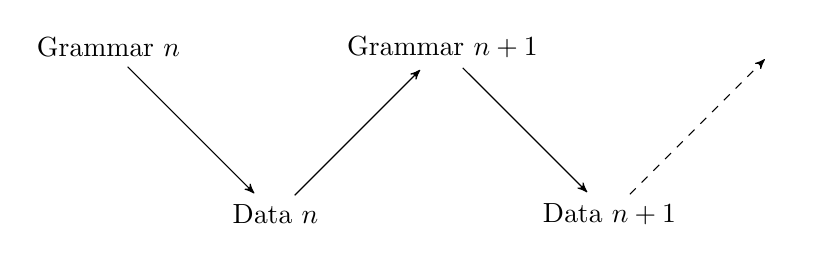
\begin{tikzpicture}[->,>=stealth',shorten >=1pt,auto,node distance=3cm]
      \node (A)      {Grammar $n$};
      \node (B) [below right of=A]  {Data $n$};
      \node (C) [above right of=B] {Grammar $n+1$};
      \node (D) [below right of=C] {Data $n+1$};
      \node (E) [above right of=D] {};
      \path[->] (A)  edge node {} (B)
      (B) edge node {} (C)
      (C) edge node {} (D)
      (D) edge[dashed] node {} (E);
    \end{tikzpicture}
  \end{center}
\end{frame}

\begin{frame}
  \frametitle{Acquisition}
  \begin{center}
    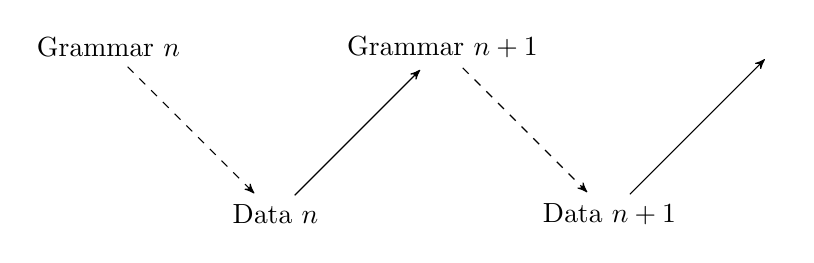
\begin{tikzpicture}[->,>=stealth',shorten >=1pt,auto,node distance=3cm]
      \node (A)      {Grammar $n$};
      \node (B) [below right of=A]  {Data $n$};
      \node (C) [above right of=B] {Grammar $n+1$};
      \node (D) [below right of=C] {Data $n+1$};
      \node (E) [above right of=D] {};
      \path[->] (A)  edge[dashed] node {} (B)
      (B) edge node {} (C)
      (C) edge[dashed] node {} (D)
      (D) edge node {} (E);
    \end{tikzpicture}
  \end{center}
\end{frame}

\begin{frame}
\frametitle{\cite{chomsky1980rules}}
\begin{columns}[T]  
   \begin{column}{.25\textwidth}
     % \begin{center}
	  \vspace{15pt}
	  \includegraphics[height=1in]{chomsky.jpg}   
     % \end{center}
   \end{column}
   \begin{column}{.7\textwidth}
      \begin{block}{}
      \begin{quote}
	   By \textbf{grammatical competence} I  mean the cognitive state that encompasses all those aspects of form and meaning and their relation.
      \end{quote}           
      \end{block}
    \end{column}
  \end{columns}
\end{frame}


\begin{frame}
  \frametitle{Use}
  \begin{center}
    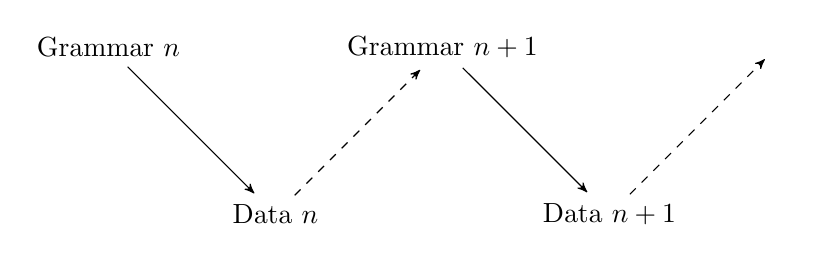
\begin{tikzpicture}[->,>=stealth',shorten >=1pt,auto,node distance=3cm]
      \node (A)      {Grammar $n$};
      \node (B) [below right of=A]  {Data $n$};
      \node (C) [above right of=B] {Grammar $n+1$};
      \node (D) [below right of=C] {Data $n+1$};
      \node (E) [above right of=D] {};
      \path[->] (A)  edge node {} (B)
      (B) edge[dashed] node {} (C)
      (C) edge node {} (D)
      (D) edge[dashed] node {} (E);
    \end{tikzpicture}
  \end{center}
\end{frame}

 

\begin{frame}
\frametitle{\cite{chomsky1980rules}}
\begin{columns}[T]  
   \begin{column}{.25\textwidth}
     % \begin{center}
	  \vspace{15pt}
	  \includegraphics[height=1in]{chomsky.jpg}   
     % \end{center}
   \end{column}
   \begin{column}{.7\textwidth}
      \begin{block}{}
      \begin{quote}
	   By \textbf{grammatical competence} I  mean the cognitive state that encompasses all those aspects of form and meaning and their relation...\textbf{Pragmatic competence} underlies the ability to use such knowledge along with the conceptual system to achieve certain ends or purposes. 
      \end{quote}           
      \end{block}
    \end{column}
  \end{columns}
\end{frame}

\begin{frame}
\frametitle{\cite{grice:1975}}
\begin{columns}[T]  
   \begin{column}{.25\textwidth}
     % \begin{center}
	  \vspace{20pt}
	  \includegraphics[height=1.2in]{grice.jpg}   
     % \end{center}
   \end{column}
   \begin{column}{.7\textwidth}
      \begin{block}{}
      \begin{quote}
	   I am, however, enough of a rationalist to want to find a basis that underlies these facts, undeniable though they may be; I would like to be able to think of the standard type of conversational practice not merely as something that all or most do \textbf{in fact} follow but as something that it is \textbf{reasonable} for us to follow, that \textbf{we should not abandon}. 
      \end{quote}           
      \end{block}
    \end{column}
  \end{columns}
\end{frame}


% \begin{frame}
% \frametitle{\cite{grice:1975}}
% \begin{columns}[T]  
%    \begin{column}{.25\textwidth}
%      % \begin{center}
% 	  \vspace{10pt}
% 	  \includegraphics[height=1.2in]{grice.jpg}   
%      % \end{center}
%    \end{column}
%    \begin{column}{.7\textwidth}
%       \begin{block}{Pragmatic Competence}
% 	\begin{itemize}
% 	     \item Beliefs
% 	    \item Preferences
% 	    \item Intentions
% 	\end{itemize}
%       \end{block}
%     \end{column}
%   \end{columns}
% \end{frame}


\begin{frame}
\frametitle{\cite{grice:1975}}
\begin{columns}[T]  
   \begin{column}{.25\textwidth}
     % \begin{center}
	  \vspace{10pt}
	  \includegraphics[height=1.2in]{grice.jpg}   
     % \end{center}
   \end{column}
   \begin{column}{.7\textwidth}
      \begin{block}{}
      \begin{quote}
	   Make your conversational contribution  such as is required, at the stage at which it occurs, by the accepted purpose or direction of the talk exchange in which you are engaged. One might label this the \textbf{Cooperative Principle}.
      \end{quote}           
      \end{block}
    \end{column}
  \end{columns}
\end{frame}

\begin{frame}
\frametitle{\cite{grice:1975}}
\begin{center}
     \includegraphics[width=2in]{cooperation-grice.png}
\end{center}
\end{frame}

\begin{frame}
\frametitle{\cite{grice:1975}}
\begin{center}
     \includegraphics[width=2in]{cooperation.png}
\end{center}
\end{frame}


\begin{frame}
\frametitle{\cite{jespersen:1917}}
\begin{columns}[T]  
   \begin{column}{.25\textwidth}
     % \begin{center}
%  	  \vspace{20pt}
	  \includegraphics[height=1.2in]{jespersen.jpg}   
     % \end{center}
   \end{column}
   \begin{column}{.7\textwidth}
      \begin{block}{The Negative Cycle}
	\begin{enumerate}
	     \item N V
	     \item N V N
	     \item V N
	\end{enumerate}
      \end{block}
    \end{column}
  \end{columns}
\end{frame}

\begin{frame}
\frametitle{\cite{jespersen:1917}}
\begin{columns}[T]  
   \begin{column}{.25\textwidth}
     % \begin{center}
%  	  \vspace{20pt}
	  \includegraphics[height=1.2in]{jespersen.jpg}   
     % \end{center}
   \end{column}
   \begin{column}{.7\textwidth}
      \begin{block}{The Negative Cycle}
	\begin{enumerate}
	     \item \textbf{N V}
	     \item \textbf{N V N}
	     \item V N
	\end{enumerate}
      \end{block}
    \end{column}
  \end{columns}
\end{frame}

\begin{frame}
\frametitle{\cite{jespersen:1917}}
\begin{columns}[T]  
   \begin{column}{.25\textwidth}
     % \begin{center}
%  	  \vspace{20pt}
	  \includegraphics[height=1.2in]{jespersen.jpg}   
     % \end{center}
   \end{column}
   \begin{column}{.7\textwidth}
      \begin{block}{The Negative Cycle}
	\begin{enumerate}
	     \item N V
	     \item \textbf{N V N}
	     \item \textbf{V N}
	\end{enumerate}
      \end{block}
    \end{column}
  \end{columns}
\end{frame}


% \subsection{Components}


% \begin{frame}
% \frametitle{\cite{jespersen:1917}}
% \begin{columns}[T]  
%    \begin{column}{.25\textwidth}
%      % \begin{center}
% % 	  \vspace{10pt}
% 	  \includegraphics[height=1.2in]{jespersen.jpg}   
%      % \end{center}
%    \end{column}
%    \begin{column}{.7\textwidth}
%       \begin{block}{The Negative Cycle}
% 	\begin{enumerate}
% 	     \item Use: N V > N V N
% 	     \item Acquisition: N V N > V N
% 	\end{enumerate}
%       \end{block}
%     \end{column}
%   \end{columns}
% \end{frame}



% \subsection{Contributions}



% 
% 
% \begin{frame}
% \frametitle{\cite{yang2000internal}}
%     \begin{center}
%         \begin{tikzpicture}
% 	  \node (A) [draw,circle,minimum size=4cm]  at (0,0) {$\alpha$};
% 	  \node (G1) [above of=A] {$G_1$};
% 	  \node [draw,circle,minimum size=4cm] (B) at (0:3cm) {$\beta$};
% 	  \node (G2) [above of=B] {$G_2$};
% 	\end{tikzpicture}         
%     \end{center}
% \end{frame}

\begin{frame}
  \frametitle{Language Change}
  \begin{center}
    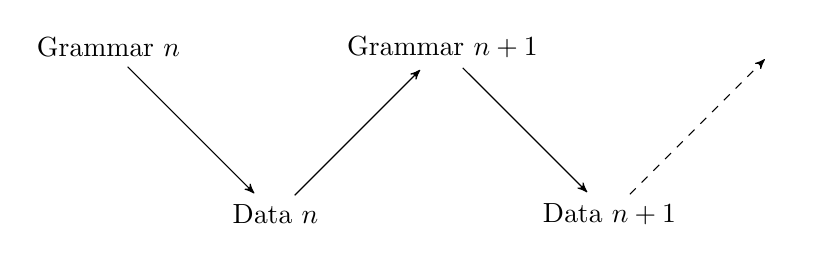
\begin{tikzpicture}[->,>=stealth',shorten >=1pt,auto,node distance=3cm]
      \node (A)      {Grammar $n$};
      \node (B) [below right of=A]  {Data $n$};
      \node (C) [above right of=B] {Grammar $n+1$};
      \node (D) [below right of=C] {Data $n+1$};
      \node (E) [above right of=D] {};
      \path[->] (A)  edge node {} (B)
      (B) edge node {} (C)
      (C) edge node {} (D)
      (D) edge[dashed] node {} (E);
    \end{tikzpicture}
  \end{center}
\end{frame}


 
\section[Background]{Background}


\begin{frame}{Background}
      \begin{enumerate}
           \item Jespersen's Cycle
	   \item Emphatic Negation
      \end{enumerate}
\end{frame}

\subsection{Jespersen's Cycle}

\begin{frame}
\frametitle{\cite{jespersen:1917}}
\begin{columns}[T]  
   \begin{column}{.25\textwidth}
     % \begin{center}
%  	  \vspace{20pt}
	  \includegraphics[height=1.2in]{jespersen.jpg}   
     % \end{center}
   \end{column}
   \begin{column}{.7\textwidth}
      \begin{block}{The Negative Cycle}
	\begin{enumerate}
	     \item N V
	     \item N V N
	     \item V N
	\end{enumerate}
      \end{block}
    \end{column}
  \end{columns}
\end{frame}


\begin{frame}
\frametitle{\cite{jespersen:1917}}
\begin{columns}[T]  
   \begin{column}{.25\textwidth}
     % \begin{center}
	  \vspace{8pt}
	  \includegraphics[height=1.2in]{jespersen.jpg}   
     % \end{center}
   \end{column}
   \begin{column}{.7\textwidth}
      \begin{block}{The Negative Cycle}
	\begin{enumerate}
	     \item N V
	     \item N V (N)
	     \item N V N
	     \item (N) V N
	     \item V N
	\end{enumerate}
      \end{block}
    \end{column}
  \end{columns}
\end{frame}

\begin{frame}
\frametitle{\cite{jespersen:1917}}
\begin{center}
\begin{tabular}{@{}lp{3cm}p{3cm}p{2.5cm}@{}}
\hline
 & Stage 1 & Stage 2 & Stage 3\\
\hline
English & ic ne secge & I ne seye not & I say not\\
& (Old English) & (Middle English) & (Early Modern English)\\
\hline
French & jeo ne dis & je ne dis pas & je dis pas \\
& (Old French) & (Middle French) & (Coloquial French) \\
\hline
\end{tabular}\label{table1}
\end{center}
\end{frame}


\begin{frame}
\frametitle{Pull-Chain}
      \begin{block}{}
      \begin{quote}
	The original negative adverb is first \textbf{weakened}, then found insufficient and therefore \textbf{strengthened}, generally through some additional word, and this in turn may be felt as the negative proper and may then in the course of time be subject to the same development as the original word.
      \end{quote}           
      \end{block}
      \begin{block}{}
      \begin{quote}
	Sometimes it seems as if the essential thing were only to increase the \textbf{phonetic bulk} of the adverb...
      \end{quote}           
      \end{block}
\end{frame}

\begin{frame}
\frametitle{Pull-Chain?}
      \begin{block}{}
	\begin{itemize}
	     \item Greek \cite{kiparsky-condoravdi:2006}
	     \item Italo-Romance \cite{posner1985}
	     \item Morphosyntactic Change
	\end{itemize}
      \end{block}
\end{frame}


\begin{frame}
\frametitle{Push-Chain}
      \begin{block}{}
      \begin{quote}
	But in most cases the addition serves to make the negative more impressive as being \textbf{more vivid or picturesque}, generally through an \textbf{exaggeration}, as when substantives meaning something very small are used as subjuncts.
      \end{quote}           
      \end{block}
\end{frame}

\begin{frame}
\frametitle{Push-Chain?}
      \begin{block}{}
	\begin{itemize}
	     \item Greek \cite{kiparsky-condoravdi:2006}
	     \item Inflation \cite{dahl:2001}
	     \item Redundancy \cite{detges-waltereit2002}
	\end{itemize}
      \end{block}
\end{frame}


% \begin{frame}{\cite{kiparsky-condoravdi:2006}}
%       \begin{block}{}
%        \begin{quote}
%         	    \textbf{Emphatic negation tends to increase} in frequency due to pragmatically motivated overuse which is characteristic of inherently bounded evaluative scales...An obligatory element cannot be emphatic, for \textbf{to emphasize everything is to emphasize nothing.}
%        \end{quote}
%       \end{block}
% \end{frame}

\begin{frame}{\cite{kiparsky-condoravdi:2006}}
\begin{columns}[T] 
   \begin{column}{.25\textwidth}
     % \begin{center}
	  \vspace{20pt}
	  \includegraphics[width=1.2in]{epic_cycle.jpg}   
     % \end{center}
   \end{column}
   \begin{column}{.7\textwidth}
      \begin{block}{}
       \begin{quote}
        	    \textbf{Emphatic negation tends to increase} in frequency due to pragmatically motivated overuse which is characteristic of inherently bounded evaluative scales...an obligatory element cannot be emphatic, for \textbf{to emphasize everything is to emphasize nothing.}
       \end{quote}
      \end{block}
    \end{column}
  \end{columns}
\end{frame}


\subsection{Emphasis}

% \begin{frame}
% \frametitle{\cite{eckardt2006}\small{\cite{krifka1995polarity}}}
%       \begin{block}{}
%       \begin{quote}
% 	Emphatic negation is the result of \textbf{emphatic focus} of an \textbf{NPI} in the scope of negation. Its pragmatic contribution to sentence meaning comes about fully compositionally.
%       \end{quote}           
%       \end{block}
% \end{frame}
% 
\begin{frame}
\frametitle{\cite{eckardt2006}\small{\cite{krifka1995polarity}}}
      \begin{block}{Interpretation}
     \begin{equation}
          \inter{E}^f = \{\inter{E}^o\}
     \end{equation}
     \begin{equation}
	  \inter{E_f}^f = \{\inter{E}^o, F_1, F_2, F_3...\}
     \end{equation}         
      \end{block}

      \begin{block}{Composition}
      \begin{equation}
          \inter{AB}^f = \{ A_i \infty B_j | A_i \in \inter{A}^f, B_j \in \inter{B}^f \}
      \end{equation}       
      \end{block}
\end{frame}

\begin{frame}
\frametitle{\cite{eckardt2006}}
    \begin{block}{Lexicon}
     \begin{equation}
	    \inter{\text{John}_f}^f = \{ \inter{\text{John}}^o,\text{ Joe, Jim}\} = \{ \text{John, Joe, Jim} \}
     \end{equation}

     \begin{equation}
	    \inter{\text{knows the number}}^f = \{ \la x . know(x, \text{the number}) \}
     \end{equation}
    \end{block}

    \begin{block}{Result}
     \begin{equation}
      \begin{split}
           \inter{\text{knows the number}}^f(\inter{John_f}^f) = \{& know(\text{John, the number}),\\& know(\text{Joe, the number}),\\& know(\text{Jim, the number}) \}
      \end{split}
     \end{equation}     
    \end{block}
\end{frame}

\begin{frame}
\frametitle{\cite{eckardt2006}}
  \begin{block}{Operator}
    \begin{equation}
      \begin{split}
         & \mathbf{emph}(S)\\  
         & asserts: \inter{S}^o \\
	 & implicates: \forall S' \in \inter{S}^f . P(\inter{S}^o) \leq P(\inter{S'}^o)
      \end{split}
    \end{equation}   
  \end{block}
    \begin{block}{Result}
    \begin{equation}
      \begin{split}
         & \mathbf{emph}(\inter{\text{John$_f$ knows the number}}^f)\\  
         & asserts: \text{John knows the number} \\
	 & implicates: \text{...of all people!}
      \end{split}
    \end{equation}   
    \end{block}
\end{frame}

\begin{frame}
\frametitle{\cite{eckardt2006}}
  \begin{block}{Combined}
    \begin{equation}
      \begin{split}
         & \mathbf{emph}(\text{John didn't drink [a single drop]}_f)\\  
         & asserts: \text{John didn't drink a single drop}\\
	 & implicates: \text{...not a glassful, not a mouthful,...!}
      \end{split}
    \end{equation}
  \end{block}
\end{frame}


\begin{frame}{\cite{fauconnier1975}}
\begin{center}
	\includegraphics[height=1in]{israel.png}   
     \end{center}
\end{frame}

\begin{frame}{\cite{kadmon-landman1993any}}

     \begin{block}{Widening}
     \ex. \a. Will there be French fries tonight?
	  \b. No, I don't have potatoes.
	  \c. Maybe just a couple I could fry in my room?
	  \d. No, I don't have any potatoes.

      \end{block}
      \begin{block}{Strengthening}
      \ex. \a. If you move, I'll shoot.
	   \b. If you budge an inch, I'll shoot.

      \end{block}
\end{frame}

\begin{frame}{\cite{austin1962}\footnotesize{\cite{lewis1970,landman1991,krifka1995polarity}}}
     \begin{center}
	\includegraphics[height=1.5in]{hexagon.jpg}   
     \end{center}
\end{frame}


\begin{frame}{\cite{austin1962}\footnotesize{\cite{lewis1970,landman1991,krifka1995polarity}}}
     \begin{center}
	\includegraphics[height=1.5in]{hex-nut.jpg}   
     \end{center}
\end{frame}





\section[Signaling]{Signaling}

\begin{frame}{Signaling}
      \begin{enumerate}
           \item Game
	   \item Equilibria
% 	   \item Dynamics
      \end{enumerate}
\end{frame}


\subsection{Signaling Games}

\begin{frame}{Structure}
\begin{block}{}
\begin{enumerate}
     \item \textbf{Sender} observes some state of the world, $t \in T$, given prior probability distribution over states, $\delta$.
     \item \textbf{Sender} chooses message, $m \in M$, based on strategy $s: T \rightarrow M$.
     \item \textbf{Receiver} interprets message with action, $a \in A$, based on strategy $r : M \rightarrow A$.
\end{enumerate}
\end{block}
\end{frame}


\begin{frame}{\cite{lewis:1969}}
\begin{columns}[T]  
   \begin{column}{.5\textwidth}
      \begin{block}{}
      \begin{quote}
	   One if by land, two if by sea.
      \end{quote}           
      \end{block}
    \end{column}
   \begin{column}{.4\textwidth}
     % \begin{center}	  
	  \includegraphics[height=1.5in]{revere.png}   
     % \end{center}
   \end{column}
  \end{columns}
\end{frame}


\begin{frame}
\tikzstyle{level 1}=[sibling distance=15cm, level distance = 4.5cm]
\tikzstyle{level 2}=[sibling distance=8cm]
\tikzstyle{level 3}=[sibling distance=4cm]
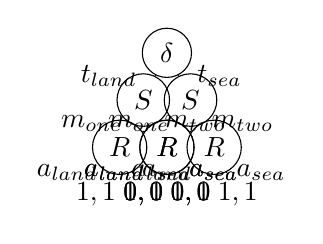
\begin{tikzpicture}[scale=.4]
%[scale=.9, level/.style={sibling distance=70mm/#1}]
\node  (z)[circle,draw]{$\delta$}
  child {node [circle,draw] (a_left) {$S$}
    child {node  [circle,draw](left_left) {$R$}
      child {node {$1,1$}        
      edge from parent
		node[left] {$a_{land}$}
		node[right] {}} 
      child {node (n){$0,0$}
      edge from parent
		node[left] {}
		node[right] {$a_{sea}$}}
    edge from parent
	node[left] {$m_{one}$}
	node[right] {}}
    child {node  [circle,draw](left_right) {$R$}
      child {node {$1,1$}        
      edge from parent
		node[left] {$a_{land}$}
		node[right] {}} 
      child {node (n){$0,0$}
      edge from parent
		node[left] {}
		node[right] {$a_{sea}$}}
    edge from parent
	node[left] {}
	node[right] {$m_{two}$}}
  edge from parent
	node[left] {$t_{land}$ $ $}
	node[right] {}
  }
 child {node [circle,draw] (a_right) {$S$}
    child {node  [circle,draw](right_left) {$R$}
      child {node {$0,0$}        
      edge from parent
		node[left] {$a_{land}$}
		node[right] {}} 
      child {node (n){$1,1$}
      edge from parent
		node[left] {}
		node[right] {$a_{sea}$}}
    edge from parent
	node[left] {$m_{one}$}
	node[right] {}}
    child {node  [circle,draw](right_right) {$R$}
      child {node {$0,0$}        
      edge from parent
		node[left] {$a_{land}$}
		node[right] {}} 
      child {node (n){$1,1$}
      edge from parent
		node[left] {}
		node[right] {$a_{sea}$}}
    edge from parent
	node[left] {}
	node[right] {$m_{two}$}}
  edge from parent
	node[left] {}
	node[right] {$ $ $t_{sea}$}
  };
\draw [dashed](left_left) to [out=35,in=-215] (right_left);
\draw [dashed](left_right) to [out=35,in=-215] (right_right);
\end{tikzpicture}
\end{frame}

% \begin{frame}
% \begin{block}{Sender}
% \begin{itemize}
%      \item Observes some state of the world, $t \in T$, given prior probability distribution over states, $\delta$.
%      \item Chooses message, $m \in M$, based on strategy $s \in [T \rightarrow M]$.
% \end{itemize}
% \end{block}
% 
% \begin{block}{Receiver}
% \begin{itemize}
%      \item Interprets message with action, $a \in A$, based on strategy $r \in [M \rightarrow A]$.
% \end{itemize}
% \end{block}
% \end{frame}

\begin{frame}{(Expected) Utilities}
\begin{block}{}
\begin{equation}
 U_{S}(t_i, a_k) = U_{R}(t_i, a_k) =
\left\{
	\begin{array}{ll}
		1  & \mbox{if } i = k \\
		0 & \mbox{else}
	\end{array}
\right.
\end{equation}\end{block}
\begin{block}{}
	\begin{equation}
	    \begin{split}
	      E[U_{S}(s,r)] &= \sum_{t} \delta (t) \cdot U_S(t, r(s(t)))\\
	      E[U_{R}(s,r)] &= \sum_{t} \delta (t) \cdot U_r(t, r(s(t)))
	    \end{split}
	\end{equation}
\end{block}
\end{frame}



\subsection{Equilibria}

\begin{frame}{\cite{nash:1951}}
\begin{columns}[T]  
   \begin{column}{.75\textwidth}
      \begin{block}{}
 A strategy profile $\langle s^*, r^*\rangle$ is a \textbf{Nash equilibrium}
if and only if:
  \begin{itemize}
   \item $\forall s \in S$, such that $s \neq s^*$, $E[U_S(s^*,r^*)] \geq
E[U_S(s,r^*)]$
  \item $\forall r \in R$, such that $r \neq r^*$, $E[U_R(s^*,r^*)] \geq
E[U_S(s^*,r)]$
  \end{itemize}
      \end{block}
      \begin{block}{}
           \emph{Something that it is \textbf{reasonable} for us to follow.} -Grice
      \end{block}

    \end{column}
    \begin{column}{.2\textwidth}
     % \begin{center}
	  \vspace{12pt}
	  \includegraphics[height=1.2in]{nash.jpg}   
     % \end{center}
     \end{column}
  \end{columns}
\end{frame}

% \subsection{Evolutionarily Stable Strategies}

\begin{frame}{\cite{maynard-smith-price:1973}}
\begin{columns}[T]  
   \begin{column}{.75\textwidth}
      \begin{block}{}
	\begin{quote}
	     An Evolutionarily Stable Strategy is a strategy that, if all the members of a population adopt it, then \textbf{no mutant strategy could invade the population} under the influence of natural selection.
	\end{quote}  
      \end{block}
    \end{column}
    \begin{column}{.2\textwidth}
     % \begin{center}
	  \vspace{12pt}
	  \includegraphics[height=1.1in]{maynard.jpg}   
     % \end{center}
     \end{column}
  \end{columns}
\end{frame}

\begin{frame}{\cite{selten:1980}}
\begin{columns}[T]  
   \begin{column}{.75\textwidth}
      \begin{block}{}
	A strategy profile $\langle s^*, r^*\rangle$ is evolutionarily stable if and only if it is a \textbf{Strict Nash equilibrium}:
	\begin{itemize}
	    \item $\forall s \in S$, such that $s \neq s^*$, $E[U_S(s^*,r^*)] > E[U_S(s,r^*)]$
	    \item $\forall r \in R$, such that $r \neq r^*$, $E[U_R(s^*,r^*)] > E[U_S(s^*,r)]$
	\end{itemize}
      \end{block}
      \begin{block}{}
           \emph{Something that it is \textbf{reasonable} for us to follow, that we \textbf{should not} abandon.} -Grice
      \end{block}

    \end{column}
    \begin{column}{.2\textwidth}
     % \begin{center}
	  \vspace{20pt}
	  \includegraphics[height=1in]{selten.jpg}   
     % \end{center}
     \end{column}
  \end{columns}
\end{frame}

\begin{frame}{Separating Equilibria}
\begin{center}
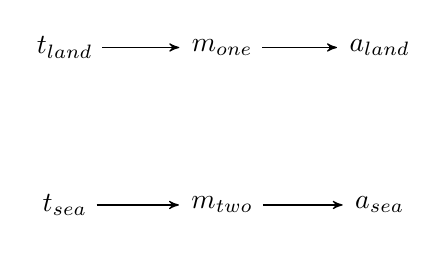
\begin{tikzpicture}[->,>=stealth',shorten >=1pt,auto,node distance=2cm]
  \node (A)      {$t_{land}$};
  \node (B) [right of=A]  {$m_{one}$};
  \node (C) [right of=B] {$a_{land}$};
  \node (D) [below of=A] {$t_{sea}$};
  \node (E) [right of=D] {$m_{two}$};
  \node (F) [right of=E] {$a_{sea}$};
\path[->] (A) edge node {} (B)
	  (B) edge node {} (C)
	  (D) edge[below] node {} (E)
	  (E) edge[below] node {} (F);
\end{tikzpicture}     

\end{center}
\end{frame}

\begin{frame}{Pooling Equilibria}
\begin{center}
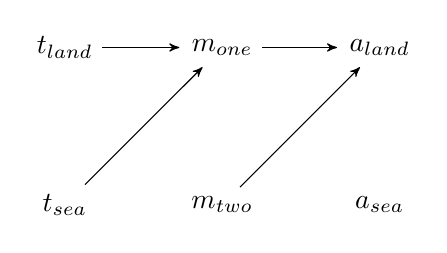
\begin{tikzpicture}[->,>=stealth',shorten >=1pt,auto,node distance=2cm]
  \node (A)      {$t_{land}$};
  \node (B) [right of=A]  {$m_{one}$};
  \node (C) [right of=B] {$a_{land}$};
  \node (D) [below of=A] {$t_{sea}$};
  \node (E) [right of=D] {$m_{two}$};
  \node (F) [right of=E] {$a_{sea}$};
\path[->] (A) edge node {} (B)
	  (B) edge node {} (C)
	  (D) edge[below] node {} (B)
	  (E) edge[below] node {} (C);
\end{tikzpicture}     
\end{center}
\end{frame}

\begin{frame}{Pooling Equilibria}
\begin{center}
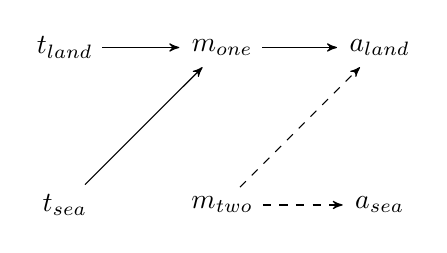
\begin{tikzpicture}[->,>=stealth',shorten >=1pt,auto,node distance=2cm]
  \node (A)      {$t_{land}$};
  \node (B) [right of=A]  {$m_{one}$};
  \node (C) [right of=B] {$a_{land}$};
  \node (D) [below of=A] {$t_{sea}$};
  \node (E) [right of=D] {$m_{two}$};
  \node (F) [right of=E] {$a_{sea}$};
\path[->] (A) edge node {} (B)
	  (B) edge node {} (C)
	  (D) edge[below] node {} (B)
	  (E) edge[dashed] node {} (C)
	  (E) edge[dashed] node {} (F);
\end{tikzpicture}     
\end{center}
\end{frame}


% \subsection{Dynamics}
% 
% \begin{frame}{\cite{taylor-jonker:1978}}
% \begin{columns}[T]  
% \begin{column}{.25\textwidth}
%      % \begin{center}
% 	  \vspace{20pt}
% 	  \includegraphics[height=1in]{ess.png}   
%      % \end{center}
%      \end{column}
%    \begin{column}{.7\textwidth}
%       \begin{block}{Replicator Equations}
% % 	Let $\mathbf{x}$ and $\mathbf{y}$ represent the composition of a sender and receiver populations respectively.
% 	\begin{equation}
% 	    \begin{split}
% 	     \dot{x}_i &= x_i(f_i(\mathbf{y}) - f(\mathbf{y}))\\
% 	      \dot{y}_i &= y_i(g_i(\mathbf{x}) - g(\mathbf{x}))	         
% 	    \end{split}
% 	\end{equation}
%       \end{block}
%     \end{column}
%   \end{columns}
% \end{frame}




\section[Cycles]{Cycles}

\begin{frame}{Cycles}
      \begin{enumerate}
           \item Game
	   \item Equilibria
% 	   \item Dynamics
      \end{enumerate}
\end{frame}

\subsection{Game}

\begin{frame}{Structure}
\begin{block}{}
\begin{itemize}
     \item \textbf{Speaker} has evidence for some standard of precision, $t \in T: [0,1]$,  given prior density function over states, $\delta$.
     \item \textbf{Speaker} chooses a form of negation, $m \in M$, based on strategy $s : \mathcal{P}_n(T) \rightarrow M$
     \item \textbf{Hearer} infers standard of precision, $a \in A$, based on strategy $r : M \rightarrow A$.
\end{itemize}
\end{block}
\end{frame}

% \begin{frame}{(Expected) Utilities}
% \begin{block}{}
%  \begin{equation}
% \begin{split}
%      U_S(t, a) &= ?\\
%   	 U_R(t, a) &= ?
% \end{split}
% \end{equation}
% \end{block}
% 
% \begin{block}{}
% 	\begin{equation}
% 	    \begin{split}
% 	      E[U_{S}(s,r)] &= \int_{T} \delta (t) \cdot U_S(t, r(s(t)))dt\\
% 	      E[U_{R}(s,r)] &= \int_{T} \delta (t) \cdot U_R(t, r(s(t)))dt
% 	    \end{split}
% 	\end{equation}
% \end{block}
% \end{frame}


\begin{frame}{}
     \begin{center}
	\includegraphics[height=3.2in]{doorbells.jpg}   
     \end{center}
\end{frame}

\begin{frame}{}
     \begin{center}
	\includegraphics[height=1.5in]{saussure.jpg}   
     \end{center}
\end{frame}

\begin{frame}{Advice!}
      \begin{block}{}
      \ex. \a. If you move, I'll shoot.
	   \b. If you budge an inch, I'll shoot.

      \end{block}
      \begin{block}{}
	 \ex. \a. That restaurant's not good.
	      \b. That restaurant's not worth a cent!

      \end{block}
\end{frame}


\begin{frame}{\cite{crawford-sobel:1982}}
\begin{center}
     \includegraphics[width=2in]{payoffgraph2.pdf} \hspace{.5cm} \includegraphics[width=2in]{payoffgraph.pdf}
\end{center}
\end{frame}

\begin{frame}{(Expected) Utilities}
\begin{block}{}
 \begin{equation}
\begin{split}
     U_S(t, a) &= -(a - t - b)^2\\
  	 U_R(t, a) &= -(a - t)^2
\end{split}
\end{equation}
\end{block}

\begin{block}{}
	\begin{equation}
	    \begin{split}
	      E[U_{S}(s,r)] &= \int_{T} \delta (t) \cdot U_S(t, r(s(t)))dt\\
	      E[U_{R}(s,r)] &= \int_{T} \delta (t) \cdot U_R(t, r(s(t)))dt
	    \end{split}
	\end{equation}
\end{block}
\end{frame}


\subsection{Equilibria}

% \begin{frame}{Equilibria}
% \begin{equation}
%  \frac{\partial}{\partial t^*}E[U_S(s, r)] = 0
% \end{equation}
% \begin{equation}
% \frac{\partial}{\partial a_1^*}E[U_R(s, r)] = \frac{\partial}{\partial a_2^*}E[U_R(s, r)] = 0
% \end{equation}
% \end{frame}

\begin{frame}{Pooling Equilibria}
\begin{block}{Always $m_1$}
 \begin{equation}
    t^* = 1
  \end{equation}
\begin{equation}
	  a_1^* = \frac{t^*}{2}
\end{equation}     
\end{block}
\end{frame}


\begin{frame}{Pooling Equilibria}
\begin{block}{Always $m_2$}
 \begin{equation}
    t^* = 0
  \end{equation}
\begin{equation}
	  a_2^* = \frac{1 + t^*}{2}
\end{equation}     
\end{block}
\end{frame}



\begin{frame}{(Partially-)Separating Equilibrium}
\begin{block}{Differentiate $m_1$ and $m_2$}
      \begin{equation}
    t^* = \frac{1}{2} - 6b
  \end{equation}
\begin{equation}
     \begin{split}
	  a_1^* &= \frac{t^*}{2}\\
	  a_2^* &= \frac{1 + t^*}{2}
     \end{split}
\end{equation}
\end{block}
\end{frame}

\begin{frame}{\cite{crawford-sobel:1982}}
     \begin{center}
	\includegraphics[height=2.5in]{bias.pdf}   
% floor(.5*(sqrt(1 + (2/b)) - 1) see CS82 p.1441
     \end{center}
\end{frame}

\begin{frame}{Push-Chain}
    \begin{center}
    \begin{tabular}{@{}cc@{}}
      \hline
       \textsc{Plain} & \textsc{Emphatic}\\
      \hline
      \textsc{n V} &  \textsc{n V}  \\
      \textsc{n V} &  \textsc{n V (n)}  \\
      \textsc{n V (n)} &  \textsc{n V n} \\
      \textsc{n V n} &  \textsc{n V n} \\
      \hline
    \end{tabular}
    \end{center}
\end{frame}


\begin{frame}{\cite{kullback-leibler1951divergence}}
  \begin{center}
       \includegraphics[width=2.5in]{kl-divergence.pdf}
  \end{center}
\begin{block}{}
\begin{equation}
     D_{KL}(P || Q) = \int_{-\infty}^{\infty} log\left( \frac{p(x)}{q(x)}  \right)p(x) dx
\end{equation}
\end{block}

\end{frame}


% \subsection{Dynamics}
% 
% 
% 
% \begin{frame}
% \begin{center}
% 
% \begin{tikzpicture}[->,>=stealth',shorten >=1pt,auto,node distance=2cm]
%       \node (A)      {$m_1$};
%       \node (B) [right of=A]  {$m_2$};
%       \node (C) [below of=A]  {$m_1$};
%       \node (D) [below of=B]  {$m_2$, $m_3$};
% %       \node (E) [draw, circle, above of=A] {$a_1$};
% %       \node (F) [draw, circle, above of=B] {$a_2$};
%       \node (E) [below of=C]  {$m_1$, $m_2$};
%       \node (F) [below of=D]  {$m_3$};
%       \node (G) [below of=E]  {$m_2$};
%       \node (H) [below of=F]  {$m_3$};
%       \path[->] (D)  edge node {} (E)
%       (A) edge node {} (C)
%       (B) edge node {} (D)
%       (C) edge node {} (E)
%       (D) edge node {} (F)
%       (E) edge node {} (G)
%       (F) edge node {} (H);
% \end{tikzpicture}
% \end{center}
% 
% \end{frame}


\begin{frame}
\frametitle{\cite{jespersen:1917}}
\begin{columns}[T]  
   \begin{column}{.2\textwidth}
     % \begin{center}
 	  \vspace{10pt}
	  \includegraphics[height=1in]{jespersen.jpg}   
     % \end{center}
   \end{column}
   \begin{column}{.8\textwidth}
      \begin{block}{The Negative Cycle}
	\begin{enumerate}
	     \item N V
	     \item N V (N)
	     \item N V N
	     \item (N) V N
	     \item V N
	\end{enumerate}
      \end{block}
    \end{column}
  \end{columns}
\end{frame}



\section[Stability]{Stability}

\begin{frame}{Stability(?)}
      \begin{enumerate}
           \item Learning
	   \item Mechanisms
	   \item Data
      \end{enumerate}
\end{frame}

\subsection{Learning}

\begin{frame}
\frametitle{\cite{yang2000internal}}
    \begin{center}
        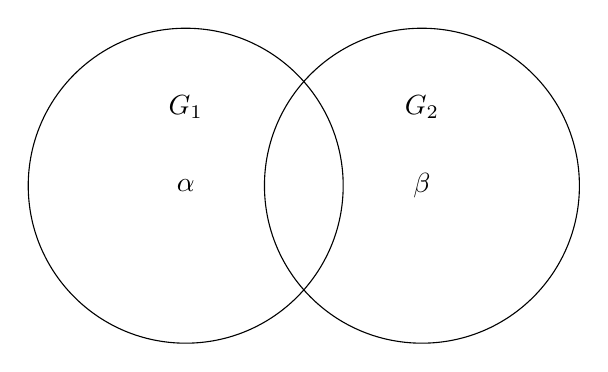
\begin{tikzpicture}
	  \node (A) [draw,circle,minimum size=4cm]  at (0,0) {$\alpha$};
	  \node (G1) [above of=A] {$G_1$};
	  \node [draw,circle,minimum size=4cm] (B) at (0:3cm) {$\beta$};
	  \node (G2) [above of=B] {$G_2$};
	\end{tikzpicture}         
    \end{center}
\end{frame}

\begin{frame}
\frametitle{\cite{yang2000internal}}

\begin{block}{Over time}
\begin{equation}
     \frac{p_t}{(1-p_t)} = \left( \frac{\alpha}{\beta} \right)^t\frac{p_0}{(1-p_0)}
\end{equation}
\end{block}

\end{frame}

\begin{frame}
  \frametitle{Language Change}
  \begin{center}
    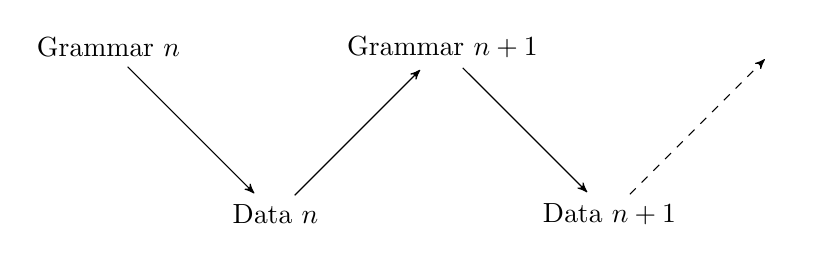
\begin{tikzpicture}[->,>=stealth',shorten >=1pt,auto,node distance=3cm]
      \node (A)      {Grammar $n$};
      \node (B) [below right of=A]  {Data $n$};
      \node (C) [above right of=B] {Grammar $n+1$};
      \node (D) [below right of=C] {Data $n+1$};
      \node (E) [above right of=D] {};
      \path[->] (A)  edge node {} (B)
      (B) edge node {} (C)
      (C) edge node {} (D)
      (D) edge[dashed] node {} (E);
    \end{tikzpicture}
  \end{center}
\end{frame}

\subsection{Mechanisms}

\begin{frame}
\frametitle{\cite{wallage2008}}
    \begin{center}
        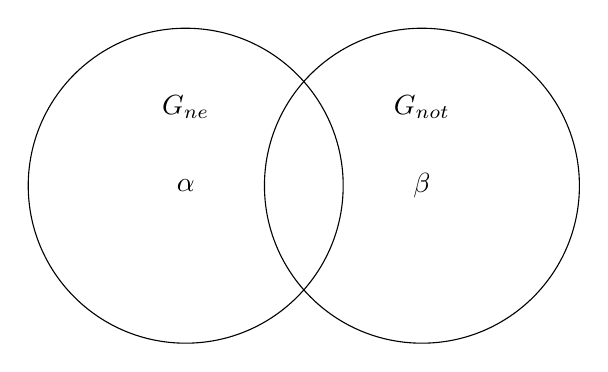
\begin{tikzpicture}
	  \node (A) [draw,circle,minimum size=4cm]  at (0,0) {$\alpha$};
	  \node (G1) [above of=A] {$G_{ne}$};
	  \node [draw,circle,minimum size=4cm] (B) at (0:3cm) {$\beta$};
	  \node (G2) [above of=B] {$G_{not}$};
	\end{tikzpicture}         
    \end{center}
\end{frame}


\begin{frame}
\frametitle{N V > N V N}
    \begin{center}
        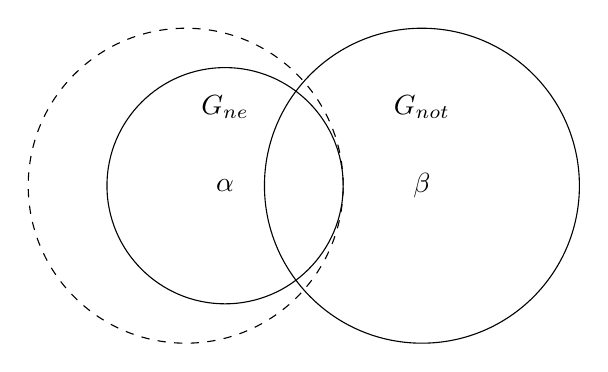
\begin{tikzpicture}
	  \node (A) [draw,circle,dashed,minimum size=4cm]  at (0,0) {};
	  \node [draw,circle,minimum size=3cm] (C) at (0:.5cm) {$\alpha$};
	  \node (G1) [above of=C] {$G_{ne}$};
	  \node [draw,circle,minimum size=4cm] (B) at (0:3cm) {$\beta$};
	  \node (G2) [above of=B] {$G_{not}$};
	\end{tikzpicture}         
    \end{center}
\end{frame}

\begin{frame}
\frametitle{N V > N V N}
    \begin{center}
        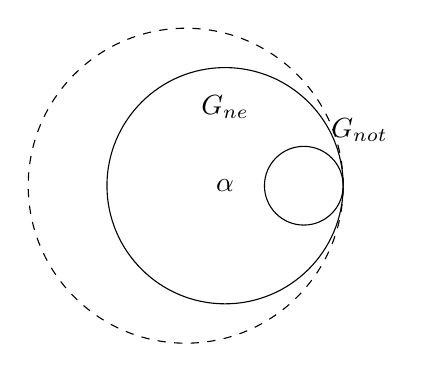
\begin{tikzpicture}
	  \node (A) [draw,circle,dashed,minimum size=4cm]  at (0,0) {};
	  \node [draw,circle,minimum size=3cm] (C) at (0:.5cm) {$\alpha$};
	  \node (G1) [above of=C] {$G_{ne}$};
	  \node [draw,circle,minimum size=1cm] (B) at (0:1.5cm) {};
	  \node (G2) [above right of=B] {$G_{not}$};
	\end{tikzpicture}         
    \end{center}
\end{frame}

\begin{frame}
\frametitle{N V > N V N}
    \begin{center}
        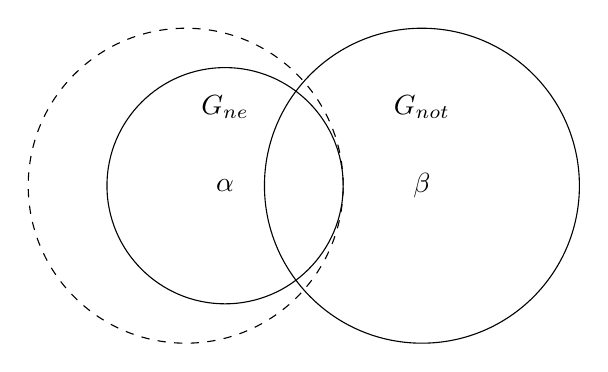
\begin{tikzpicture}
	  \node (A) [draw,circle,dashed,minimum size=4cm]  at (0,0) {};
	  \node [draw,circle,minimum size=3cm] (C) at (0:.5cm) {$\alpha$};
	  \node (G1) [above of=C] {$G_{ne}$};
	  \node [draw,circle,minimum size=4cm] (B) at (0:3cm) {$\beta$};
	  \node (G2) [above of=B] {$G_{not}$};
	\end{tikzpicture}         
    \end{center}
\end{frame}

\subsection{Data}

\begin{frame}
\frametitle{\cite{wallage2008}}
    \begin{center}
\footnotesize{
\begin{tabular}{@{}ccccccc@{}}
\hline
 & Main Clauses & & &Subordinate Clauses &  &\\
\hline
Period & \emph{ne} & \emph{ne...not} & \emph{not} & \emph{ne} & \emph{ne...not} & \emph{not}\\
\hline
1150-1250 & 91 & 152 & 3  & 279 & 112 & 4  \\
1250-1350 & 48 & 329 & 48 & 87 & 147 & 15  \\
1350-1420 & 3 & 108 & 935 & 17 & 115 & 905  \\
1420-1500 & 1 & 12 & 928  & 7 & 4 & 821  \\
\hline
\end{tabular}
}
\end{center}
\end{frame}

\begin{frame}
\frametitle{\cite{wallage2008}}
\begin{center}
\footnotesize{
\begin{tabular}{@{}cccccccc@{}}
\hline
& \emph{if}-clauses  & & &In scope of negation &    &\\
\hline
Period & \emph{ne} & \emph{ne...not} & \emph{not} & \emph{ne} & \emph{ne...not} & \emph{not}\\
\hline
1150-1250 & 33 & 10 & 0  & 33 & 3 & 0  \\
1250-1350 & 12 & 8 & 3  & 19 & 6 & 2  \\
1350-1420 & 9 & 5 & 64  & 14 & 8 & 55  \\
1420-1500 & 2 & 1 & 51  & 4 & 1 & 43  \\
\hline
\end{tabular}
}
\end{center}
\end{frame}

\begin{frame}{\cite{wallage2008}}
\begin{center}
\begin{tabular}{@{}cccccc@{}}
\hline
Period & $\alpha$ & $\beta$ & $\frac{\beta}{\alpha}$ & \emph{ne...not}\\
\hline
1150-1250 & 370 & 40  & .108 & 277\\
1250-1350 & 137 & 65 & .474 & 490\\
1350-1420 & 75 & 1799 & 23.986 & 236\\
1420-1500 & 51 & 1704 & 33.411 & 18\\
\hline
\end{tabular}
\end{center} 
\end{frame}

\begin{frame}
\begin{center}
 \includegraphics[height=2in]{ecay.png}
\end{center}
\tiny{*Thanks to Aaron Ecay for queries and code.}
\end{frame}

\begin{frame}
\frametitle{Actuation}

\begin{block}{Over time}
\begin{equation}
     \frac{p_t}{(1-p_t)} = \left( \frac{\alpha}{\beta} \right)^t\frac{p_0}{(1-p_0)}
\end{equation}
\end{block}

\begin{block}{Misperception}
\begin{equation}
     P(not) = P(ne...not)*\epsilon
\end{equation}     
\end{block}

\end{frame}

\begin{frame}
\frametitle{N V > N V N}
    \begin{center}
        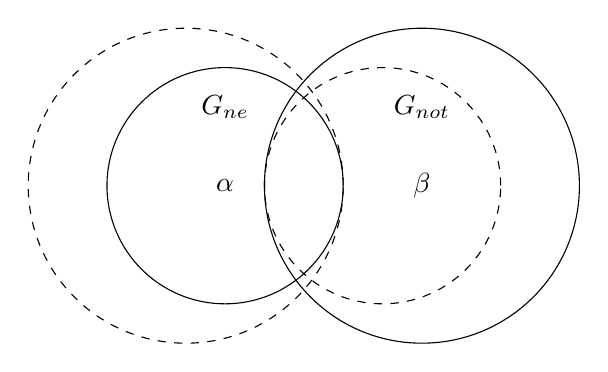
\begin{tikzpicture}
	  \node (A) [draw,circle,dashed,minimum size=4cm]  at (0,0) {};
	  \node [draw,circle,minimum size=3cm] (C) at (0:.5cm) {$\alpha$};
	  \node (G1) [above of=C] {$G_{ne}$};
	  \node (O) [draw,circle,dashed,minimum size=3cm]  at (0:2.5cm) {};
	  \node [draw,circle,minimum size=4cm] (B) at (0:3cm) {$\beta$};
	  \node (G2) [above of=B] {$G_{not}$};
	\end{tikzpicture}         
    \end{center}
\end{frame}


\begin{frame}
\frametitle{\cite{jespersen:1917}}
\begin{columns}[T]  
   \begin{column}{.2\textwidth}
     % \begin{center}
 	  \vspace{10pt}
	  \includegraphics[height=1in]{jespersen.jpg}   
     % \end{center}
   \end{column}
   \begin{column}{.8\textwidth}
      \begin{block}{The Negative Cycle}
	\begin{enumerate}
	     \item N V
	     \item N V (N)
	     \item N V N
	     \item (N) V N
	     \item V N
	\end{enumerate}
      \end{block}
    \end{column}
  \end{columns}
\end{frame}



\section*{Conclusion}

% \subsection{Future Directions}


\begin{frame}
  \frametitle{Language Change}
  \begin{center}
    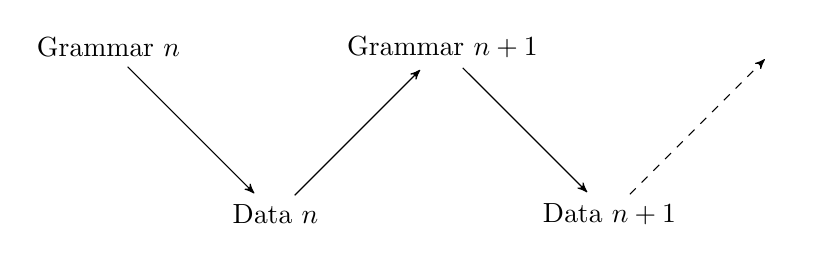
\begin{tikzpicture}[->,>=stealth',shorten >=1pt,auto,node distance=3cm]
      \node (A)      {Grammar $n$};
      \node (B) [below right of=A]  {Data $n$};
      \node (C) [above right of=B] {Grammar $n+1$};
      \node (D) [below right of=C] {Data $n+1$};
      \node (E) [above right of=D] {};
      \path[->] (A)  edge node {} (B)
      (B) edge node {} (C)
      (C) edge node {} (D)
      (D) edge[dashed] node {} (E);
    \end{tikzpicture}
  \end{center}
\end{frame}

\begin{frame}{Future Directions}
\begin{block}{}
 \begin{itemize}
  \item \emph{Common prior assumption} \cite{harsanyi:1967}.
  \item Theoretical implications of prior.
  \item Empirical evidence about prior.
 \end{itemize}
\end{block}

\begin{block}{}
 \begin{itemize}
  \item More articulated theory of change \cite{frisch1997,wallage2008}.
  \item Detailed analysis of Middle English data.
  \item Comparison to parallel change in French.
 \end{itemize}
\end{block}
\end{frame}


\begin{frame}
\begin{center}
\huge Thanks!
\end{center}
\end{frame}


% 
\begin{frame}[allowframebreaks]{References}
\bibliographystyle{plainnat}
\footnotesize{\bibliography{ahern}}
\end{frame}




\end{document}
